\documentclass{article}
\usepackage{amsmath}
\usepackage{graphicx}
\bibliographystyle{unsrt}

\title{Implementation of an Implicit PIC Method in minEPOCH}
\author{T. Goffrey}


\begin{document}

\maketitle

This document contains a description of the implicit particle-in-cell (PIC) method implemented within the minEPOCH mini-app, as part of the ExCALIBUR-NEPTUNE project. The purpose of this document is to provide an explanation for the design choices made during the development, and to make suggestions for future research. For instructions on compiling and running the code, users should consult the included README document. 

\section{Explicit PIC Algorithm}
A brief explanation of time-explicit PIC methods is included in order to assist the reader. For a full description many good references (e.g. \cite{birdsall} \cite{EPOCH}) are available. The electromagnetic PIC method solves Maxwell's equations coupled to particles moving under the influence of the Lorentz force. Typically the electric and magnetic fields ($\vec{E}, \vec{B}$)are evolved using the finite difference time domain (FDTD) method:

\begin{align}
  \vec{E}^{n+1/2} &= \vec{E}^n + \frac{\Delta t}{2}\left(c^2 \nabla \times \vec{B}^n - \frac{\vec{J}^n}{\epsilon_0}\right) \\
  \vec{B}^{n+1/2} &= \vec{B}^n - \frac{\Delta t}{2}\left(\nabla \times \vec{E}^{n+1/2}\right) \\
  \vec{B}^{n+1} &= \vec{B}^{n+1/2} - \frac{\Delta t}{2}\left(\nabla \times \vec{E}^{n+1/2}\right) \\
  \vec{E}^{n+1} &= \vec{E}^{n+1/2} + \frac{\Delta t}{2}\left(c^2 \nabla \times \vec{B}^{n+1} - \frac{\vec{J}^{n+1}}{\epsilon_0}\right) \\
\end{align}

Note that this four-step process can be written more efficiently as a two-step leap-frog scheme. The four-step process has the advantage of having fields defined at the same time.
Field components are defined on the staggered Yee \cite{Yee} mesh, which as well as meaning all finite differences needed for the field update are centered, also conserves $\nabla \cdot \vec{B} = 0$.

Each time-step the particle momenta $\vec{p} = \gamma m \vec{a}$)are updated according to the Lorentz force:

\begin{equation}
  \vec{p}^{n+1} = \vec{p} + q \Delta t\left(\vec{E}^{n+1/2}_p + \vec{v}^{n+1/2} \times \vec{B}^{n+1/2}_p\right)
\end{equation}

where $\vec{E}^{n+1/2}_p, \vec{B}^{n+1/2}_p$ are the electric and magnetic fields evaluated at the particle half time-step position respectively. Several methods exist to update the momenta, of which the Boris method \cite{Boris} is a very common choice.

The particle position, similarly to the field update is typically written as a split leapfrog scheme

\begin{align}
  \vec{x}^{n+1/2} &= \vec{x}^n + \frac{\Delta t}{2} \vec{v}^n \\
  \vec{x}^{n+1} &= \vec{x}^{n+1/2} + \frac{\Delta t}{2} \vec{v}^{n+1} \\
\end{align}

where the momentum update is carried out between the two steps. The process of updating the particle position and momentum is commonly referred to a ``particle push''. In order to calculate the electric and magnetic fields at the particle positions, particle shape functions are used, such that the field experiences by a particle is calculated as a weighted average of the field at surrounding grid points. In principle the same method can be used to calculate the current density at grid points,

\begin{equation}
  \vec{j}_{\mathrm{Grid}} = \sum_{\mathrm{particles}} W_p^G \vec{v}_p q_p,
\end{equation}

where $W_p^G$ represents the particle weighting to each grid point. However, this method can lead to an electric field which violates Gauss' law. Instead, a method originally due to Esirkepov \cite{esirkepov}, and later generalised by Villasenor and Buneman \cite{villasenor} is used. Rather than calculating the current density from particle moments, the current density is calculated to be consistent with charge conservation,

\begin{equation}
  \frac{\partial}{\partial t}\rho = - \nabla \cdot \vec{j},
\end{equation}

which automatically ensures Gauss's law is satisfied.

\subsection{Timestep Constraints}

The electromagnetic solver requires (in 1D)

\begin{equation}
  \Delta t \leq \frac{\Delta x}{c}
\end{equation}

for stability. Explicit PIC codes also require the plasma frequency to be resolved,

\begin{equation}
  \Delta t \leq \frac{2 \pi}{\omega_{pe}}.
\end{equation}

Note that if the Debye length is resolved then the timestep constraint due to the electromagnetic solver is the most restrictive.

Finally we note at this stage that the finite size and number of explicit PIC codes results in a non-smooth field, $\delta \vec{E}$, which acts to heat the plasma. This is referred to as self-heating.

\section{Implicit Method}

To overcome the stability constraints and self-heating of explicit PIC codes, many variants of implicit and semi-implicit PIC codes have been designed. The time-implicit method within minEPOCH is based on the method of Markidis and Lapenta \cite{markidis}. The complete set of equations (Maxwell's equations and the particle push) are solved using the Crank-Nicolson method. In order to reduce the memory requirements of the method the Jacobian-free Newton-Krylov (JFNK) method is used to solve the resulting non-linear equations. Furthermore, to reduce the size of the linear system the particle enslavement technique, as described in \cite{markidis},\cite{chen} is used.

The field components are stored on the same staggered (Yee) mesh as the explicit field solver in minEPOCH. This ensures that the relations:

\begin{equation}
  \nabla \cdot \nabla \times \vec{a} = 0
\end{equation}

and

\begin{equation}
  \nabla \cdot \left(\vec{a} \times \vec{b}\right) = \vec{b}\cdot \left(\nabla \times \vec{a}\right) - \vec{a}\cdot\left(\nabla\times\vec{b}\right)
\end{equation}

hold true on the discrete mesh. This is required for energy conservation. Note that whilst necessary for these relations to hold true, it is not sufficient for the electromagnetic solver to be energy conserving - explicit minEPOCH does not conserve energy, even in a vacuum.

The implicit method implemented in minEPOCH conserves the total energy of the system:

\begin{equation}
  E = \sum_{\mathrm{cells}} \frac{V\epsilon_0}{2} \left(\vec{E}^2 + c^2 \vec{B}^2\right) + \sum_{\mathrm{particles}} \frac{1}{2}m\vec{v}^2,
\end{equation}

rather than the relativistically correct formula for particle energy, therefore energy conservation measurements reported in this document will be defined as above.

\subsection{Particle Pushing}

The particle push in the implicit version of minEPOCH is as presented in \cite{markidis}:

\begin{align}
  \tilde{\vec{v}} &= \vec{v}^n + \frac{q \Delta t}{2 m}\vec{E}_p \\
  \bar{\vec{v}} &= \frac{\tilde{\vec{v}} + \frac{q \Delta t}{2 m}\left(\tilde{\vec{v}} \times \vec{B}_p + \frac{q \Delta t}{2 m}\tilde{\vec{v}} \cdot \vec{B}\vec{B}\right)}{1 + \frac{q^2\Delta t^2 \vec{B}^2}{4m^2}}\\
  \vec{v}^{n+1} &= 2 \bar{\vec{v}} - \vec{v}^n \\
  \vec{x}^{n+1} &= \vec{x}^n  + \bar{\vec{v}} \Delta t
\end{align}

The key requirement for energy conservation is that the magnetic field rotation does not change the energy of the particle (as it shouldn't, of course), and that the electric field acceleration is properly time centered, such that the change in kinetic energy is given by:

\begin{equation}
  \Delta T = m \bar{\vec{v}} q \bar{\vec{E}}_p \Delta t
\end{equation}

This is sufficient for energy conservation, as long as the current used for the electric field update is given by

\begin{equation}
  \bar{\vec{J}} = \sum_{\mathrm{particles}} q \bar{\vec{v}} W_p^G.
\end{equation}

As the particle enslavement method is used, a particle push must be completed for every residual evaluation of the field solve. Due to the dependence of the acceleration on the particle position, the equation for each particle is non-linear, and must be solved iteratively. A fixed-point iteration is used for each particle, and terminates when the corrections to velocity and position obey:

\begin{align}
  \left| \Delta \vec{v}\right| &\leq 10^{-8} c \\
  \left| \Delta \vec{x}\right| &\leq 10^{-8}.
\end{align}

These requirements worked well in testing, but may need adjusting in future.


\subsection{Gauss Law}

The previous section has an important caveat - that in order to conserve total energy, it is not possible to use the same methods as explicit codes to conserve charge, and thus not violate Gauss' law.
Two methods were considered to alleviate this problem. The first is the method of Chen et al \cite{chen}. The method uses the fact that if you use a higher order shape function to represent the charge density, and substep the particle push such that the particle pauses as it moves between cells, it is possible to conserve charge. However, from a computational perspective, this introduces a per-particle (sub) time-step, and (likely) increases the number of particle pushes required. Independent of the increased computational cost and complexity, this method only works for low order particle shape functions, indeed below the minimum recommended accuracy of suggested for laser-plasma studies suggested in \cite{EPOCH}. Of course, this might not hold true for (e.g.) MCF applications, but the method was not considered further. However, there is an option for substepping in implicit minEPOCH, which may be beneficial in cases where the time-step is much greater than the inverse of the plasma frequency.

Rather than conserve charge directly, minEPOCH instead uses the method described in \cite{markidis} (amongst many other references), which diffuses errors in Gauss's law away to the boundary, the speed of which is controlled by a parameter specified by the user. This does stop the accumulation of errors in Gauss' law. However, the presence of non-zero errors, as well as the extra terms in Maxwell's equations to remove them, alters the dispersion relation of electromagnetic waves. Careful research, using a realistic test problem is required to evaluate if this is problematic, and possible tuning of the speed of the diffusion of errors may be required.

\subsection{Results}

A complete study of the implicit minEPOCH method is beyond the scope of this document. However, we present two sets of results. The first is a comparison of run time relative to the explicit solver in minEPOCH, as a function of CFL number for the provided two-stream instability. Where possible we compare to published results.

\subsection{Runtime}

The runtime of the implicit version of minEPOCH, relative to the explicit version, on a single core using the two stream instability set-up is shown in Figure ~\ref{fig:CFL}. The best relative performance is seen for a CFL value of 12.0, although this is still $\sim 5.8$ times slower than the explicit code. The closest direct comparison of the two methods in the literature is in the work of Lapenta \cite{lapenta}, which includes (in Table 1) a similar comparison for 1D versions of the two algorithms. Here the implicit method is $\sim 34$ times slower than the explicit, but run with the same timestep. The same comparison with minEPOCH shows the implicit version to be $\sim 22.5$ times slower. We note that the calculations here used a non-linear tolerance of $10^{-2}$ and a linear tolerance of $10^{-1}$, which could impact run time comparisons, but did show similar levels of energy conservation to the explicit code for all CFL numbers considered. Indeed the error in energy conservation is (almost) independent of timestep used.

\begin{figure}[h]
  \caption{Plot of runtime for implicit minEPOCH, normalised by the equivalent explicit runtime.}
  \centering
  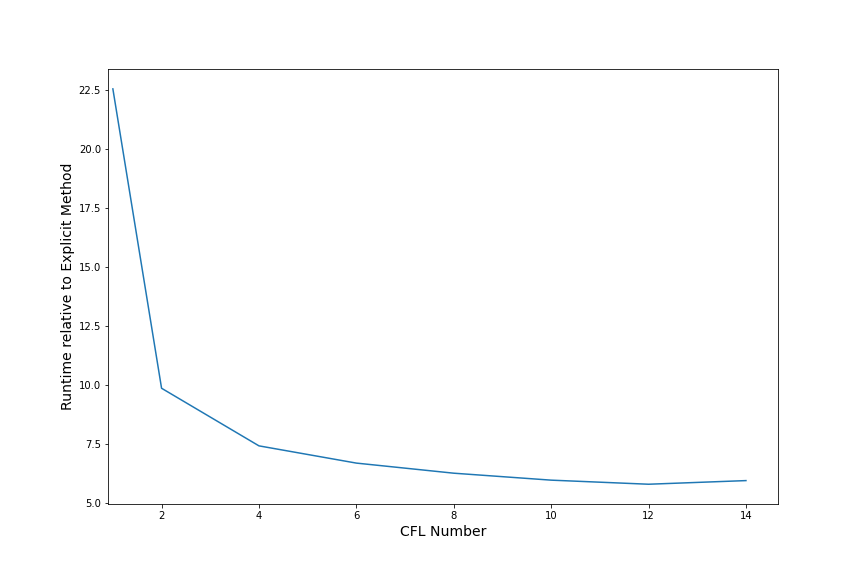
\includegraphics[width=0.9\textwidth]{CFL.png}
  \label{fig:CFL}
\end{figure}

\subsection{Energy Conservation}

The conservation of energy error for a number of different non-linear tolerances, using the implicit algorithm of minEPOCH is shown in Figure ~\ref{fig:energy}. For all implicit runs shown the linear tolerance was set to $10^{-2}$, and a CFL number of $1.0$ was used. As expected the level of conservation of energy improves with a more restrictive non-linear tolerance, with all runs except for the least stringent ($10^{-2}$) showing better energy conservation than the standard time-explicit algorithm. Direct comparison with published data is complicated by the use of dimensionless numbers in reference implementations, making like-for-like comparisons of tolerances non-trivial, but the qualitative behaviour in minEPOCH matches published data.

\begin{figure}[h]
  \caption{Plot of fractional error in total energy for implicit minEPOCH, with varying non-linear tolerances. The equivalent data set for the explicit algorithm is included for reference.}
  \centering
  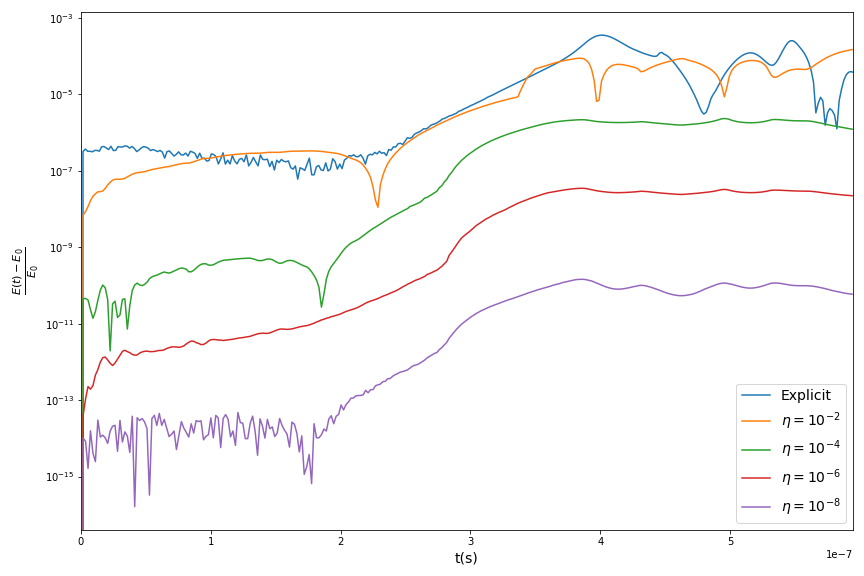
\includegraphics[width=0.9\textwidth]{energy.png}
  \label{fig:energy}
\end{figure}


\section{Recommendations and Future Work}

The clearest requirement for future research is the need to design a preconditioner for the JFNK system, without which when studying like-for-like problems the explicit PIC method will always be preferable, unless the PIC self-heating is severe. As no explicit matrix is formed a likely possible option would be ``physics based preconditioning'', which involves solving an approximate system of equations, and using that approximate solution as a preconditioning operator. One notable example involves a fluid based preconditioner for an electrostatic PIC code \cite{chacon_pic_pbp}, although many other examples of physics based preconditioning exist within the wider literature \cite{chacon20032d}, \cite{viallet2016jacobian}, \cite{park2009physics}. It is possible that some gains can be made by exploiting scaling of the system. However, it's likely that optimum scaling would be problem dependent, and thus isn't explored here. Similarly, it's possible that modifying/reducing the convergence requirements of the particle push could drastically improve performance.

Another area which is beyond the scope of this proposal, but should be considered in the future is the impact of the divergence of errors in Gauss's law. As previously mentioned these errors likely impact the dispersion relation of electromagnetic waves. For the problems considered here these errors were not problematic, however that may not hold true for all cases. Different rates of error diffusion, combined with different particle substepping, and their impact on the results should be investigated.

There are of course many other possibilities. Due to the short length of the project it has not been possible to combine the implicit method with multiple/more complex particle pushes. In principle this would not require much modification to the code (existing pushes would have to be modified to make the final particle update optional, for example), but such approaches would be very experimental, and might need careful formulation in order for the scheme to remain energy conserving, or even stable.

The code delivered has been designed as a first implementation of an implicit PIC code for the Neptune project, and opens up a number of potentially interesting avenues of research. Despite the required future research mentioned above the tool is already or practical purpose in investigating regimes where the self heating of explicit PIC codes would render their application impractical. Comparisons to published results appear to show the current implementation is either similar to or superior to previous applications of the algorithm.

\bibliography{implicit}

\end{document}
